\documentclass[fleqn]{ILASSEurope_2026_Paper_Format}



\begin{document}
\title{Title of Paper for the ILASS Europe 2026 Conference}

\doi{}
% \doi{http://dx.doi.org/10.4995/ILASS2017.2017.*&***}
\vspace{1mm}
\author{First Author$^{*\text{1}}$, Firstname Surname$^{\text{2}}$, Last Author$^{\text{2}}$}
\vskip 5mm
\address{$^{\text{1}}$ Name of the Research Group, Department/Institute, University/Company, Country\\
$^{\text{2}}$ Division of Combustion Physics, Department of Physics, Lund University, Sweden\\
\vskip 2pt
{\corresponding{*Corresponding author:
\href{mailto:a.author@university.eu}{\textstyleInternetlink{a.author@university.eu}}}}}
\vspace{5mm}
\section*{Abstract}
This template illustrates the formatting of full-length papers for ILASS Europe 2025 proceedings. Please do not change any formatting, such as margins. The abstract should be no longer than 250 words. The main Title, the name of the Authors and of their institutes are “Centred” text with words starting with capital letters. The main text is “Justified” (make sure that it’s not “Aligned Left”).  The Font of the text is Arial Nova and the Font size equals to: 

- 14 pt. for the main Title written in Bold

- 11 pt. for the Author' Names and their respective affiliations

- 11 pt. for the top-level headings of each section written in Bold (Heading 1)

- 10 pt. for the second-level headings of each section written in Bold (Heading 2)

- 10 pt. for the Main Text

- 10 pt. for the Figure captions written in Italic

\vspace{5mm}
\textbf{Keywords:} Up to 90 characters max including spaces, to make sure it remains on a single line.
\vspace{5mm}

\section*{Introduction}
The typical length of an ILASS Europe 2025 paper should be up to 8 pages. Your first manuscript must be submitted in PDF file format before April 4th, 2025. The maximum file size must not exceed 10 MB.
\vspace{5mm}
\section{Main first section (Heading 1)}
The spacing between each section is 5 mm. Each section inserted between the introduction and the conclusion are numbered. Top-level headings (Heading 1) are numbered 1, 2, 3, for example, and second-level headings (Heading 2) are numbered 1.1, 1.2, 1.3.

\begin{figure}[h]
    \vspace{6pt}
    \centering
    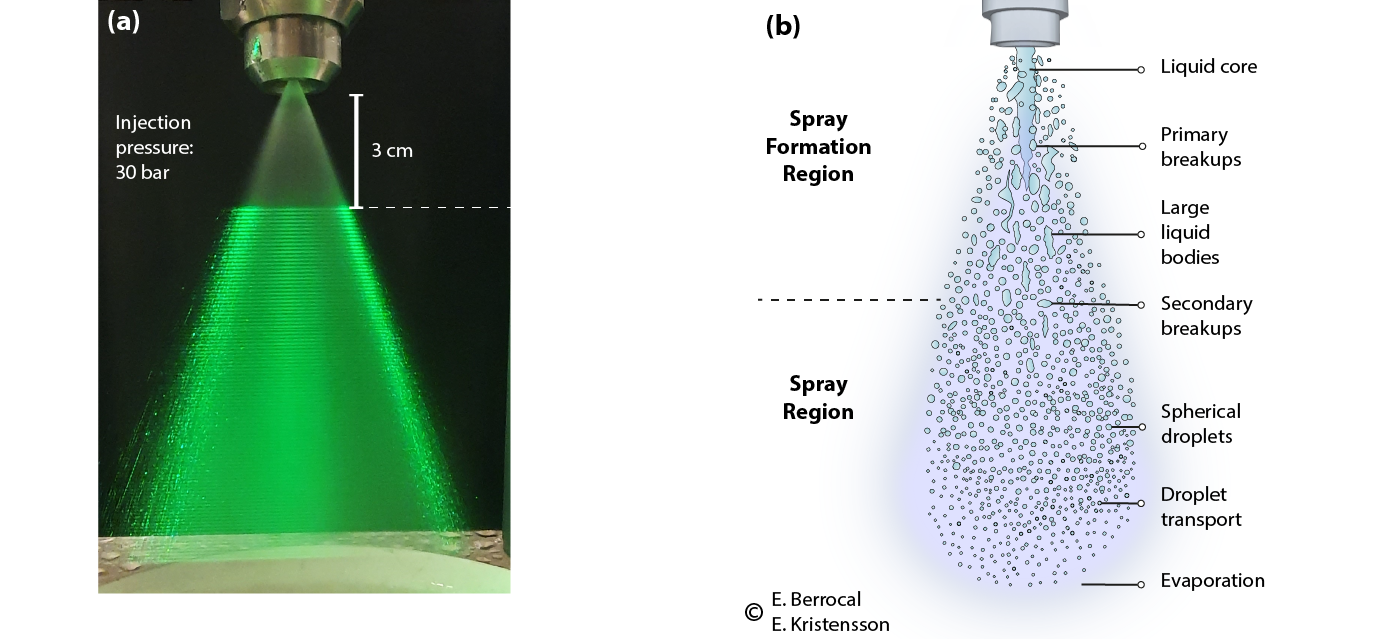
\includegraphics[width=.9\linewidth]{drawing.png}
    \centering
    \caption{Example of a figure. (a) is a picture of a hollow cone spay. (b) describes liquid atomization. Caption font size 10, italic and centred}
    \label{fig:drawing}
\end{figure}

\subsection{Sub-section (Heading 2)}
The spacing between each sub-section is 1 line. It is recommended to insert figures on the bottom or on the top of pages.

\subsection{Sub-section (Heading 2)}
The example in Figure \ref{fig:drawing} shows how to include a figure into the text. You should use 1 blank line before and after the figure. The same applies to tables. Use the table example format presented below. 

\begin{table}[h]
\centering
\caption{Example of a table. Caption font size 10, italic and centred.}
\vspace{6pt}
\begin{tabular}{|c|c|c|c|}
\hline\hline
\rule{0pt}{1.1em} & Column 1 & Column 2 & Column 3 \\\hline\hline
\rule{0pt}{1.1em} Row 1 & 5 & 34 & 67 \\\cdashline{1-4}
\rule{0pt}{1.1em} Row 2 & 6 & 45 & 75 \\\cdashline{1-4}
\rule{0pt}{1.1em} Row 3 & 7 & 46 & 64  \\\hline
\end{tabular}
\label{tab:template}
\end{table}


\bigskip
\section{Main second section}
Adequately name the headlines of each paragraph and/or add new ones. Equations should be left-aligned, with the equation number in parentheses in sequential order, right-justified, as in the below equation. The spacing between text and equation is a line of size 6 pt.
\begin{equation}\label{eq:BL-Law}
I_f/I_i = \exp(-N\cdot\sigma_e\cdot L)
\end{equation}
Equations should be referred to by equation numbers (Eq. \ref{eq:BL-Law}). All symbols should be printed in italics or otherwise according to conventional practice, both in the equations and in the text. 


\vspace{5mm}
\section*{Conclusions}
Must be inserted.
\vspace{5mm}
\section*{Acknowledgements}
Can be inserted if needed (not mandatory)
\vspace{5mm}
\section*{Nomenclature}
Can be inserted if needed (not mandatory)
\begin{tabbing}
\hspace*{1.18 cm}  \= \hspace*{4 cm}  \kill
$a$ \> acceleration [m s$^{-2}$]    \\
$F$ \> force [N]\\
$m$ \> mass [kg]
\end{tabbing}

\section*{}
References should be indicated in the text by full sized numbers enclosed within square brackets. The referencing style follows Optica's (formerly OSA) bibliography convention. Use the correct formats for e.g., journals \cite{Roth:22}, books \cite{LEFEBVRE2017} and symposium proceedings \cite{Lampa:11}. 


\bibliographystyle{refsTemplate}
\bibliography{refs}




\end{document}
